% !TeX root = ../thuthesis-example.tex

\chapter{背景知识}
本章对社群发现的基本概念、可恢复性、与有理论保证的算法进行简要介绍,作为我们研究的
基础。
\section{社群发现的数学模型}\label{sec:community_detection}
\newglossaryentry{cd}{name=社群发现, description={Community detection}}

\gls{cd}(\glsdesc{cd}) 虽然没有严格的数学定义,但公认的做法是
\newglossaryentry{graph}{name=图, description={graph}}
将现实世界的社群建模成\gls{graph}(\glsdesc{graph})结构,在图结构上进行社群发现。社群根据其属性
是否随时间变化可分为静态社群和动态社群,本文研究的是静态社群,它可以用
静态图来建模,以下简称图。
一个图结构$G$ 由节点集 $V$ 和边的集合 $E$ 组成,可记为 $G(V,E)$。
根据边是否有方向可将图分为有向图和无向图。无向图可以看成是每条边
有两个方向,从而针对有向图设计的社群发现算法也可以用到无向图上面来。
此外,根据边是否有权值可将图分为有权图和无权图。有权图中节点 $i$
和节点 $j$ 之间的权值可以用 $w_{ij}$ 表示。若有权图有方向,
则 $w_{ij}$ 可以不等于 $w_{ji}$。
无向图可以看成是每条边
的权值是1,从而针对有权图设计的社群发现算法也可以用到无权图上面来。

社群发现算法根据发现的社群是否重叠可分为两类,本文研究的是非重叠的
社群发现算法,即$V$可以分为互不重叠的若干子集。

\section{基于最小化平均误差的图分割算法}
不同的社群发现算法根据自己的标准寻找社群结构,这给一般意义上的比较造成了困难。
在本节中我们介绍的社群发现算法采用的标准叫做最小化平均误差。
这个概念最早是日本学者永野清仁于2010年提出\cite{mac},但其数学形式
在研究图强度这一概念时已被提出 \cite{cunningham1985optimal}。
在这里我们采用其最为广泛的形式,即针对带权的有向图的社群发现算法。
\begin{equation}\label{eq:IP}
  \lambda_1 := \min_{\P \in \Pi'}\frac{ f[\P] }{  \abs{\P} - 1 } 
\end{equation}
在式 \eqref{eq:IP} 中,
\newglossaryentry{not:partition}
{
  type=notation,
  name={$\P$},
  description={$V$的一个分割,
  也即  $P=\{C_1, \dots, C_k\},
  \cup_{i=1}^k C_i=V$}
}
$\P$ 表示 \glsdesc{not:partition}。
$\abs{\mathcal{P}}$ 表示集合 $\P$ 中元素的个数。
$\Pi$ 是 $V$ 上所有分割的集合而 $\Pi'=\Pi\backslash\{V\}$ 表示 $\Pi$
除去 $V$本身.
作用在$V$的子集$C$上的函数$f$
表示$C$和 $C$的补集 $V\backslash C$ 之间边的权值之和,即
$f(C)=\sum_{i \not\in C, j\in C, (i,j) \in E} w_{ij}$。
而作用在$V$的分割$\P$上的函数 $f[\P]$ 则是$f$分别作用$\P$中每一个元素之和。
即 $f[\P]=\sum_{C \in \P} f(C)$。有了如上的符号解释,
式 \eqref{eq:IP} 即不难理解,它表示各分割之间所有边的和对分割总数的平均值。

式 \eqref{eq:IP} 实际给出了一个社群发现的标准,对于扁平化的社群而言,
最小值$\lambda_1$ 对应的社群为
分割$\P^*$的子集。

下面介绍如何求解 $\lambda_1$ 及其对应的分割$\P^*$。永野清仁 \cite{mac} 的研究指出,
求解 \eqref{eq:IP} 等价于求解下面的组合优化问题
\begin{align}\label{eq:hlambda}
  h(\lambda) &= \min_{\P \in \Pi'} f[\P] - \abs{\P} \lambda 
  \end{align}
其中 $\lambda$ 是一个非负实数。
式 \eqref{eq:hlambda} 解的结构可以由一系列嵌套的分割
来描述,即存在正整数$k$,使得式 \eqref{eq:hlambda} 的解
为:
\begin{equation}\label{eq:PSP_structure}
  h(\lambda) = \begin{cases} h_{\P_0}(\lambda) & 0\leq \lambda < \lambda_1 \\
  h_{\P_i}(\lambda) & \lambda_i \leq \lambda < \lambda_{i+1} \textrm{ for } i = 1, \dots, k-1 \\
  h_{\P_k}(\lambda) & \lambda \geq \lambda_k
  \end{cases}
\end{equation}
在式 \eqref{eq:PSP_structure} 中,$\lambda_1, \dots, \lambda_{k-1},
\lambda_k$ 是递增的数列,而 $h_{\P}(\lambda)=f[\P]-|\P|\lambda$。
对于分割 $\P_0, \dots, \P_k$ 来说,
它们也有一个序关系。我们称分割 $P$ 是 $Q$ 的一个细分,
如果 $\forall C \in P, \exists C' \in Q, s.t.\, C\subset C'$,
并记为 $P \preceq Q$。基于细分的此种定义,我们有:
$\P_k \preceq \dots \preceq \P_1 \preceq \P_0$。
其中 $\P_0=\{V\}$ 而 $\P_k=\cup_{i=1}^n \{ i\}$。

在得到 $h(\lambda)$ 的表达式后,
我们指出 式 \eqref{eq:IP} 和
\eqref{eq:PSP_structure} 中的$\lambda_1$ 取值
相同,因此我们用了相同的符号。而 $\P^*=\P_1$。
从而式 \eqref{eq:IP}的解可以从式 \eqref{eq:PSP_structure}
的解中获得。

下面举一个简单的例子来解释上面的结论。
\begin{example}\label{ex:psp}
考虑一个带权的有向图$G(V,E)$,其结构
如图 \ref{fig:example_directed} 所示。
试求解该图的主分割序列。
\end{example}
\begin{figure}
  \centering
  \begin{subfigure}[b]{0.5\linewidth}
  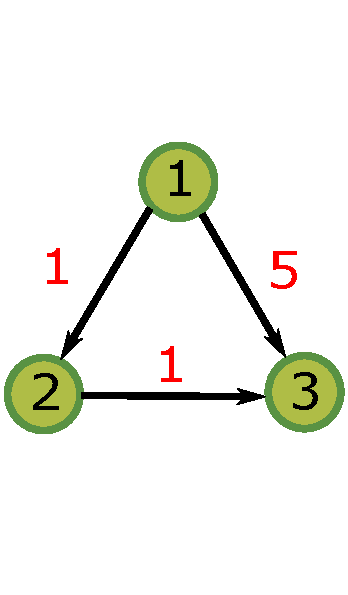
\includegraphics[width=\textwidth]{example_directed.pdf}
  \caption{一个有三个节点的带权有向图}
  \label{fig:example_directed}
  \end{subfigure}~
  \begin{subfigure}[b]{0.5\linewidth}
    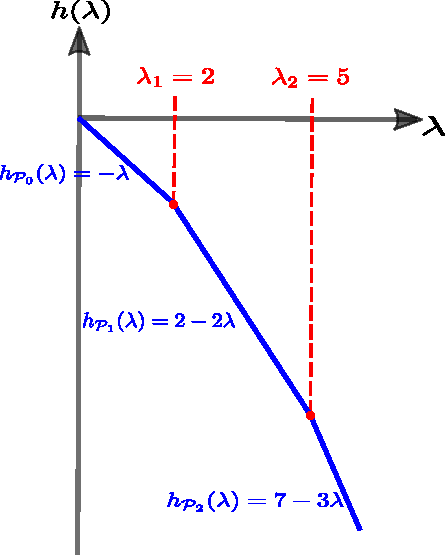
\includegraphics[width=\textwidth]{dt.pdf}
    \caption{$h(\lambda)$ 的图像}
    \label{fig:dt}
    \end{subfigure}  
\end{figure}

因为
$G$ 包含的节点只有3个,可以使用枚举法计算对应的 $h(\lambda)$
函数,其函数图像如图 \ref{fig:dt} 所示。其中
$\P_0=\{ \{1,2,3\} \}, \P_1 = \{\{1,3\}, \{2\} \},
\P_2 =\{\{1\},\{2\},\{3\} \}$。
从图\ref{fig:dt} 中可以看到,在这个简单的例子中
$h(\lambda)$
是一个分段线性函数,对于一般的图$G$对应的
$h(\lambda)$ 也是如此。

因此,基于最小平均分割的方法,\ref{fig:example_directed}
中的图将被 划分成 $\P^*=\P_1$,即节点1和3被分成一类,
而节点2单独分成1类,这符合我们的直觉。

对于一般的图,其节点数目可能很多,此时用枚举法计算
$h(\lambda)$ 变得不可行。幸运的是,计算
$h(\lambda)$ 有多项式时间的算法。下面对\cite{mac}中描述的
方法进行介绍。
\subsection{主分割序列}
我们把这一方法称为 PSP 算法
\footnote{该方法最早由
印度学者 纳拉亚南 在 1991 年提出 \cite{narayanan}
},
其中
PSP 是 principal sequence of partition 的缩写,译为
主分割序列。
    
求解 \eqref{eq:PSP_structure} 只需得到在每一个
分界点处对应的 $\lambda$ 和 分割$\P$ 即可。
考虑到 $\P_k \preceq \dots \preceq \P_1 \preceq \P_0$
,
我们有 $|\P_0| \leq |\P_1| \dots \leq |\P_k|$,
即随着 $\lambda $ 的增大,线性函数的斜率逐渐增大。
这从图 \ref{fig:dt} 中也可以得到印证。
利用这一特点,我们基于分治的思想采用算法\ref{alg:psp}
获得分割序列。

\renewcommand{\algorithmicrequire}{\textbf{输入:}\unskip}
\renewcommand{\algorithmicensure}{\textbf{输出:}\unskip}

\begin{algorithm}
  \caption{求解主分割序列的算法 (PSP算法)}
  \label{alg:psp}
  \small
  \begin{algorithmic}[1]
    \REQUIRE 图$G$
    \ENSURE 序列 $L=[\lambda_1, \dots, \lambda_k]$
    和 $\mathcal{Q}=[\P_0, \dots, \P_k]$.
    \STATE \textbf{L}  $\leftarrow []$.
    \STATE $Q\leftarrow \{V\}, P \leftarrow \{ \{i \} | i \in V\}$
    %\STATE $\mathbf{PSP}= [Q, P]$
    \STATE \texttt{Split}$(Q,P)$
    \STATE 对 $L$ 和 $\mathcal{Q}$
    按从小到大排序 \footnotemark
    \FUNCTION{\texttt{Split}$(Q,P)$}
     \STATE\label{alg:lambda} $\lambda' =
     {1 \over \abs{P} - \abs{Q}} (f(P)-f(Q))$
     \STATE\label{alg:lambda_plus} $h' = {1 \over \abs{P} - \abs{Q}}(\abs{P} f(Q) - \abs{Q} f(P))$
     \STATE\label{alg:lambda_f} $(\tilde{h}, P') = \texttt{DT}(G,\lambda')$
     \IF{$\tilde{h} = h'$}
       \STATE\label{algorithme:terminer} insert $\lambda'$ to $\mathbf{L}$
     \ELSE
       \STATE insert $P'$ to $\mathcal{Q}$
       \STATE\label{algorithme:gauche} \texttt{Split}$(Q, P')$
       \STATE\label{algorithme:droit} \texttt{Split}$(P',P)$
     \ENDIF
    \ENDFUNCTION
  \end{algorithmic}
\end{algorithm}
\footnotetext{$\mathcal{Q}$
中按集合的大小排序}

在算法\ref{alg:psp}第\ref{alg:lambda_f}行,
函数 \texttt{DT} 是用来求解 式\ref{eq:hlambda} 获得最优值
$\tilde{h}$ 和最优值对应的分割 $P'$。

在算法 \ref{alg:lambda}、\ref{alg:lambda_plus} 行,
求解 $(\lambda', h')$ 相当于在二维 $(\lambda, h)$
平面上计算直线
$h = f[P] - |P| \lambda $
和 $h = f[Q] - |Q| \lambda $ 的交点。假设 $P, Q$ 对应的
分界点分别是 $\lambda_P, \lambda_Q$(约定 $\{V\}$ 对应 0,
$\{\{i\}|i\in V\}$ 对应 $+\infty$),那么根据几何直观
$\lambda_Q \leq \lambda' \leq \lambda_P$。
紧接着,\ref{algorithme:gauche} 行的调用对应在
$[\lambda_Q, \lambda']$
区间范围内寻找剩余的分界点,而
\ref{algorithme:droit} 行的调用对应在
$[\lambda', \lambda_P]$
区间范围内寻找剩余的分界点。最后,
\ref{algorithme:terminer} 行表明
$[\lambda_Q, \lambda_P]$ 内没有分界点,无需再调用
\texttt{Split} 函数。

如前所述,函数 \texttt{DT}
(Dilworth truncation,迪尔沃思截断\footnote{采用迪尔沃思截断
这个名称是沿用了文献\cite{mac}中的称谓})
是用于求解式\eqref{eq:hlambda}的算法,它实际上是一种贪心算法,
由算法\ref{alg:dt} 给出。

\begin{algorithm}
  \caption{迪尔沃思截断算法}\label{alg:dt}
  \begin{algorithmic}[1]
  \REQUIRE 图 $G$ 和 $\lambda$
  \ENSURE 分割 $\P$ 和 $h$
  \STATE
  $V^0 = \emptyset, x $ 是 $n$ 长的向量\footnotemark,
  $\mathcal{A} = \{\}$
  \FOR{$l=1, 2, \dots, n$}
  \STATE $V^l = \{l\} \cup V^{l-1}$
  \STATE\label{alg:tight} 计算 $x^* = \displaystyle\min_{ A: l \in A \subseteq V^l} f(A)- x(A)$。
   $T^l$ 是达到此最小值的集合,并且 $x_l \leftarrow x^* - \lambda$。 
    \STATE $U^l = T^l \cup [\cup \{A | A \in \mathcal{A}, A \cap T^l \neq \emptyset\}] $
  \STATE $\mathcal{A} = \{U^l\} \cup \{A | A \in \mathcal{A}, A \cap T^l = \emptyset \}$
  \ENDFOR
  \STATE $\P^* = \mathcal{A}, h_{\lambda} = x(V)$
  \end{algorithmic}
  \end{algorithm}
\footnotetext{$n$ 是图$G$中节点的个数}

算法\ref{alg:dt}涉及到一种新的运算记号$x(A)$,
这里 $x$ 表示一个向量而 $A$ 是一个集合
$x(A)$ 定义为 $\sum_{i \in A} x_i$。
此外,采用\cite{pin}中的方法,我们可以把\ref{alg:tight} 行中的最优化
问题转化成有向图上的最大流问题。
具体而言,
针对 $\displaystyle\min_{ A: l \in A \subseteq V^l} f(A)- x(A)$,
我们首先构造一个图$G'$包含节点$V'=\{0, 1, 2, \dots, l\}=\{0\} \cup V^l$。
节点 $0$ 是相对新加入的,作为最大流算法的源节点。
而$l$是目标节点。图$G'$中有向边的权值有如下定义:
\begin{equation}\label{eq:wij_prime}
  w'_{ij} = \begin{cases}
    \max\{0, -x_{i}\} & \textrm{ if } i = 0 \\
    \max\{0, -x_{i}\} + w_{il} & \textrm{ else if } j = l \\
    w_{ij} & \textrm{ otherwise }
  \end{cases}
\end{equation}

按照定义式 \eqref{eq:wij_prime}, 源节点0和目标节点j
之间的权值为零,即两节点间没有边相连。
基于定义好的图$G'$和$s=0,t=l$,我们求解如下
标准的最小割问题:
\begin{equation}\label{eq:mincut}
  \beta = \min_{A \subseteq V^l: l\in A }
  c(V' \backslash A, A)
\end{equation}

达到式\eqref{eq:mincut}
最小值的集合即是 $T^l$,并且$x^*$和 $\beta$
有如下关系式:
\begin{equation}\label{eq:beta_alpha}
  \beta = x^* + \sum_{x_v > 0, 1\leq v < l} x_v
\end{equation}


\subsection{参数化的最大流算法}
最大流算法用于解决网络流中从一点到另一点的最优运输路径的问题。
其中一类基于前置推送-标签重贴(push-relabel) \cite{Goldberg1988} 的算法
具有良好的效率。如果要解一系列的最大流问题并且这一系列的问题
之间有一定的关联性,重复调用最大流算法显然不是最优的选择。
基于这种考虑,有学者提出了参数化的最大流算法\cite{Gallo1989}用于求解
具有特殊结构的一系列的最大流问题。下面对参数化的最大流算法
进行简单的介绍。

首先让我们回顾一下最大流问题。
考虑一有向图$G(V,E)$。其节点集$V$
中包含两个特殊的节点:源节点$s$
和目标节点$t$。对每一对有向边
$(u,v)$存在一个非负的容量函数
$c(u,v)$。如果$u,v$之间没有有向边
定义$c(u,v)=0$。
最大流问题是求解流量函数
$f(u,v)$,使得$\sum_{v\in V} f(v,t)$
最大。流量函数需要满足如下约束
\begin{align}
  f(u, v) \leq c(u, v) \textrm{ for } (u, v) \in V \times V \\
  f(u, v) = -f(v, u) \textrm{ for } (u, v) \in V \times V \\
  \sum_{v \in V} f(u,v) = 0 \textrm{ for } v\in V\backslash\{s, t\}
\end{align}
最大流和形如式\eqref{eq:mincut}所示的最小割问题
互为对偶问题。因此求解最大流问题的算法也可以
用于求解最小割问题。

参数化的最大流算法考虑的问题是在最大流问题的
基础上,假设$c(s,v)$ 
是关于$\lambda$的增函数
且$c(v, t)$是$\lambda$的减函数,
分别记为
$c_{\lambda}(s,v)$ 和 $c_{\lambda}(v, t)$。
对于一系列的$\lambda_1 < \dots < \lambda_k$,
我们可以得到 $k$ 个最大流问题。参数化的最大流算法
即基于前置推送-标签重贴算法,通过保留
在$\lambda_{i-1}$上的计算状态并用于下一步的初始化,
以及适当地使用并行化的技术,使得计算$k$ 个最大流问题
的时间复杂度和只计算一个最大流问题近似相等。
\citet{kolmogorov} 提出一种方法,将求解式\ref{eq:hlambda}
转化为求解n次参数最大流问题。
这种方法与算法\ref{alg:dt}的思路不一样,
因为其基于参数化最大流,
我们称之为PMF算法
\footnote{PMF 是 parametric maximal flow 的缩写}。

\section{随机块模型}\label{sec:sbm}
随机块模型是我们研究社群发现问题主要使用的概率统计模型,我们将在
本小节对其进行简要介绍。与之相关的,我们将介绍随机块模型的精确恢复问题,从而引出误差率的概念;
此外,我们将对随机块伊辛模型这一工作进行简要介绍,该工作构成了我们第\ref{chap:sibm}章研究的基础。
最后,我们还介绍了与我们研究有关的两个社群发现算法。

\subsection{随机块模型及其精确恢复问题}\label{sec:exact_recovery}
\newglossaryentry{sbm}{name=随机块模型, description={Stochastic Block Model}}
\newacronym{acr:sbm}{SBM}{Stochastic Block Model}
\gls{sbm}(\gls{acr:sbm})是社群发现问题中最常用的统计模型之一
\cite{holland1983stochastic, abbe2017community}。
它提供了一个基准人工数据集来评估不同的社群检测算法
并启发了许多社群检测任务算法的设计 \cite{fortunato2010community}。

我们首先定义一些常用的符号。随机图仍用符号$G$表示,
其节点集 $V=\{1,\dots, n\}$ 简写成 \gls{not:n_bracket}。
\newglossaryentry{not:n_bracket}
{
  type=notation,
  name={\ensuremath{[n]}},
  description={表示集合$\{1,\dots, n\}$}
}
每个节点的标签为 $X_i$,
\newglossaryentry{not:W}
{
  type=notation,
  name={\ensuremath{W}},
  description={循环群,即$\{1, \omega, \dots, \omega^{k-1}\}$,$k=2$时$\omega=-1$}
}
从 \gls{not:W} $= \{1, \omega, \dots, \omega^{k-1}\}$中取值。
为方便后续讨论,这里我们给$W$赋予群的结构,让它成为一个阶为$k$的循环群,
即$\omega^k=1$。
\newglossaryentry{not:Wn}
{
  type=notation,
  name={\ensuremath{W^n}},
  description={$W$的$n$次笛卡尔积}
}
\gls{not:Wn} 表示 \glsdesc{not:Wn}。 

\newacronym{acr:ssbm}{SSBM}{Symetric Stochastic Block Model}
下面给出有$k$个社群的对称的随机块模型
(\gls{acr:ssbm})
的定义, 
	\begin{definition}[有$k$ 个社群的 SSBM]\label{def:SSBM}
	令 $0\leq q<p\leq 1$, $V=[n]$ 且
  $X=(X_1,\dots,X_n)\in W^n$。 对任意的 $u\in W$,
  $X$ 满足约束
  $|\{v \in [n] : X_v = u\}| = \frac{n}{k}$。
	如果下面两个条件满足,
  则称随机图 $G$ 是通过 $\SSBM(n,k,p,q)$ 模型产生的。 
	\begin{enumerate}
	\item 若 $X_i=X_j$, $G$ 在 节点 $i$ 和节点 $j$之间存在边的概率是 $p$; 
 若 $X_i \neq X_j$,  在 节点 $i$ 和节点 $j$之间存在边的概率是 $q$。
	\item 每条边的存在与否相互独立。
	\end{enumerate}
\end{definition}

在定义 \ref{def:SSBM} 中,注意到 $p>q$,
说明同社群之间的节点有边相连的概率更大,而
属于不同社群的节点之间有边相连的概率较小。

为进一步解释随机块模型,
我们定义随机变量 $Z_{ij}:=\bf{1}[\{i,j\} \in E(G)]$,
它是表示节点$i$和节点$j$之间是否存在边的指示函数。
给定节点的标签向量 $X$, 
\newglossaryentry{Bernoulli_distribution}{name=伯努利分布, description={Bernoulli distribution}}
$Z_{ij}$ 服从 \gls{Bernoulli_distribution},
\newglossaryentry{not:expectation}
{
  type=notation,
  name={$\E[\cdot]$},
  description={数学期望}
}
其 \glsdesc{not:expectation}值为
\begin{equation}
\E[Z_{ij}] =
\begin{cases}
p & \textrm{ if } X_i = X_j \\ 
q & \textrm{ if }  X_i \neq X_j
\end{cases}
\end{equation}

则 有 $n$ 个节点的随机图 $G$ 
被 
随机变量 $Z:=\{Z_{ij}, 1\leq i<j\leq n\}$ 完全确定。
这里 每一个 $Z_{ij}$ 是相互独立的。
$Z$ 的分布函数可以写为:
\begin{align}\label{eq:mle_sibm}
P_G(G)&:=P_G(Z = z| X=x) \\
&= p^{\sum_{x_i = x_j}
z_{ij}}q^{\sum_{x_i \neq x_j} z_{ij}} 
\cdot (1-p)^{\sum_{x_i = x_j} (1-z_{ij})}
(1-q)^{\sum_{x_i \neq x_j} (1-z_{ij})}
\label{eq:GmL}
\end{align}
\newglossaryentry{mle}
{name=最大似然估计,
description={Maximum likelihood estimation}}
若 参数 $p, q$ 已知,
通过求
式\eqref{eq:GmL} 的最大值
我们可以获得节点标签的估计$\hat{X}$,此即利用
\gls{mle}
%\footnote{Maximum Likelihood, 缩写为 ML}。
做社群发现。
\newglossaryentry{not:cGn}
{
  type=notation,
  name={$\cG_n$},
  description={所有包含$n$个节点的图的集合}
}

这里顺便介绍一个后文中会用到的符号 \gls{not:cGn},它表示
\glsdesc{not:cGn}。
由概率分布的归一化的性质可得,
$P_G(\cG_n) = \sum_{G\in \cG_n}P_G(G)=1$.
\newacronym{acr:ml}{ML}{Maximum Likelihood}

不加说明的情况下,\gls{mle} 算法 是无约束的。但在
定义\ref{def:SSBM} 的假设下,
还有一个额外的约束,即 $X$ 每一类的标签数量是严格相等的。
在这个约束下最大化式\eqref{eq:GmL} 我们可以得到一个等价
的优化问题--$k$类的最小割问题。
其形式为:
\begin{equation}\label{eq:minimum_k_cut}
  \min \sum_{ \{i,j\} \in E} (1-\delta(x_i, x_j))
\end{equation}
这里,示性函数 $\delta(x,y)$ 定义为:
\glsdesc{not:deltaxy}。
\newglossaryentry{not:deltaxy}
{
  type=notation,
  name={$\delta(x,y)$},
  description={当 $x=y$ 时,$\delta(x,y) = 1$; 当 $x\neq y$,$\delta(x,y)=0$}
}

\newglossaryentry{planted}{name=植入性分割模型, description={Planted partition model}}
当$k=2$时,式\eqref{eq:minimum_k_cut} 即为 \gls{planted},
是图论中经典的NP难的二分问题之一。


随机块模型的精确恢复是指某社群发现算法用在随机块模型上可以将
每个节点的类别都正确地分出来。因为随机块模型具有随机性,
这里正确的分出来是指当图的节点数目趋于无穷大时,以概率1正确。
为给出精确恢复严格的数学定义,需要引入如下置换的符号。


我们用 $S_k$ 表示 $W$  上所有的置换函数, 
$f$ 是 定义在 $W$ 上的置换函数
并且可以通过逐元素作用的方式
扩展到 $W^n$ 上。
对于任意 $\sigma \in W^n$,
定义集合 $S_k(\sigma):=\{f(\sigma)| f\in S_k\}$。
此外,我们定义两个$W^n$中的向量的距离为
\newglossaryentry{not:dist}
{
  type=notation,
  name={$\Dist(\sigma, \sigma')$},
  description={两个$W^n$中的向量的距离,即$|\{i\in[n]:\sigma_i\neq \sigma'_i\}|$}
}
\gls{not:dist}
$=|\{i\in[n]:\sigma_i\neq \sigma'_i\}|$,
其中 $\sigma,\sigma'\in W^n
$。
\begin{example}
当 $n=2$ 且 $k=2$ 时,
$\sigma=(1, \omega) \in W^2$;
$\omega^0 = 1$; $\omega \cdot \omega = \omega^2 = 1$;
令 $f$ 是一个$W$上映射,定义为
$f(1) = \omega$ 且 $f(\omega)=1$,
则 $f \in S_2$ 且 $f(\sigma) = (\omega, 1)$;
$\Dist(\sigma, f(\sigma)) = 2$;
$S_k(\sigma) = \{\sigma, f(\sigma)\}$; 且
$S_k^c(\sigma) = W^2 \backslash S_k(\sigma)
=\{(1, 1), (\omega, \omega)\}$。
\end{example}

给定 随机块模型,精确恢复问题可以正式定义如下:
\newglossaryentry{exact_recovery}{name=精确恢复, description={Exact Recovery}}
\begin{definition}[SBM 中的\gls{exact_recovery}] \label{def:SSBMR}
给定节点标签 $X$, 随机图 $G$ 从 $\SSBM(n,k,p,q)   $ 模型中采样。
一个社群发现算法$\hat{X}$ 相当于从已知的$G$中估计$X$,也被称做$X$
的估计量。称该算法
可精确恢复$X$,如果
\begin{equation}\label{eq:Pa_hat_X}
P_a(\hat{X}):=P(\hat{X} \in S_k(X)) \to 1 \textrm{ 当 }\, n \to \infty
\end{equation}
\end{definition}

在上述定义中, 记号 $\hat{X} \in S_k(X)$ 表示
我们只能获得相对于真实标签$X$的置换意义下的恢复结果。
因为没有一个类别的基准,
这种情况在无监督学习领域比较常见。
式\eqref{eq:Pa_hat_X}中记号 $P_a(\hat{X})$
被叫做 估计量 $\hat{X}$ 的
准确概率。
\begin{remark}\label{rem:metric_exact_recovery}\,
  \begin{enumerate}
    \item 令 $P_e(\hat{X}) = 1 - P_a(\hat{X})$
    表示错误概率。
    定义\ref{def:SSBMR} 也可以写成当$n\to \infty$
    时,
    $P_e(\hat{X}) \to 0$。
  \item  此外,我们要指出的是, 对给定的图 $G$, 估计量$\hat{X}$可以是确定性的也
  可以是随机的。
  对于随机算法, $\hat{X} \in S_k(X)$ 发生的概率 应该理解
  为 $\sum_{G \in \cG_n} P_G(G) P_{\hat{X}|G}(\hat{X} \in S_k(X))$。 
  对于确定的图,这个概率是 $P_G(\hat{X} \in S_k(X))$。  
  \end{enumerate}
\end{remark}

在定义\ref{def:SSBMR}中,精确恢复也称强恢复。强恢复是相对于弱恢复
而言的,前者要求所有节点都要分对,而后者只要求分对节点的比率收敛到1即可。
关于这两种恢复条件近年来涌现大量相关的研究工作,
因为我们的工作只涉及强恢复,
下面对一些和强恢复有关的重要结论进行逐一介绍。

设$a>b>0$,针对两个社群($k=2$)且$p=\A,q=\B$的情形。
Abbe \cite{abbe2015exact} 和 Mossel
\cite{mossel2016} 分别独立的研究发现了最大似然算法
精确恢复误差的变化规律。
因为最大似然算法相当于理论最优的估计量,他们的成果可总结为如下定理:
\begin{theorem}\label{thm:sbm2_phase_transition}
设 $P_e=P(\hat{X} \neq \pm X)$: 当 $n \to \infty$,
对于 $\SSBM(n,2,\A, \B)$ 模型,
有如下两种情形:
	\begin{enumerate}
		\item $\sqrt{a} - \sqrt{b} > \sqrt{2}$时,
    $P_e \to 0$, 存在算法满足精确恢复的要求;
		\item $\sqrt{a} - \sqrt{b} < \sqrt{2}$时,
    $P_e \to 1$, 没有算法可实现精确恢复。
	\end{enumerate}
\end{theorem}
定理\ref{thm:sbm2_phase_transition} 揭示了
具有2个社群结构的SBM模型在精确恢复度量下的相变规律,
该结论很快被Abbe 推广到$k>2$的情形
\cite{abbe2015community},由定理
\ref{thm:sbmk_phase_transition} 给出。
该结果可以视为一般的SBM
精确恢复条件的一个特例。

\begin{theorem}\label{thm:sbmk_phase_transition}
  对于 $\SSBM(n,k,\A, \B)$ 模型,当条件
  \begin{equation}\label{eq:abk}
    \sqrt{a} - \sqrt{b} > \sqrt{k}
  \end{equation}   
  满足时,
  精确恢复可实现,
  而当$\sqrt{a} - \sqrt{b} < \sqrt{k}$时,
  没有算法可实现精确恢复。
\end{theorem}
\newglossaryentry{hellinger}{name=海林格距离, description={Hellinger distance}}
\begin{remark}
  Abbe 在文章中指出,定理 \ref{thm:sbmk_phase_transition}
  给出的结论和 \gls{hellinger} (\glsdesc{hellinger})有关。
  对于两个$\R^d$中的向量$u,v$,它们的
  海林格距离 
  的平方定义为
  \begin{equation}
    H^2(u,v) = \frac{1}{2}
    \sum_{i=1}^d (\sqrt{u_i} - \sqrt{v_i})^2
  \end{equation}
  若定义向量 $u= (\frac{a}{k}, \frac{b}{k})$,
  $v =  (\frac{b}{k}, \frac{a}{k})$,。
  则
  $\sqrt{a} - \sqrt{b} > \sqrt{k}$ 的条件
  可改写成
  $H(u, v) > 1$,其中
  \begin{equation}\label{eq:Hellinger_abuv}
    H(u,v)=\frac{\sqrt{a} - \sqrt{b}}{\sqrt{k}}    
  \end{equation}
  上面介绍的是Abbe 引入的切尔诺夫-海林格距离的定义,
  但他在文章中使用的距离度量仅是正的测度而不是随机变量间的,该解释略显生硬。
\end{remark}

\subsection{随机块-伊辛模型}\label{sec:ising}
\begin{figure}
	\centering
	\begin{subfigure}{0.5\textwidth}
		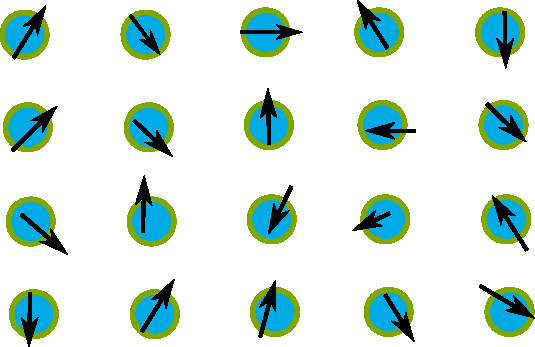
\includegraphics[width=0.7\textwidth]{Tlarge.pdf}
		\caption{$T>T_c$, random spins}
	\end{subfigure}~
	\begin{subfigure}{0.5\textwidth}
		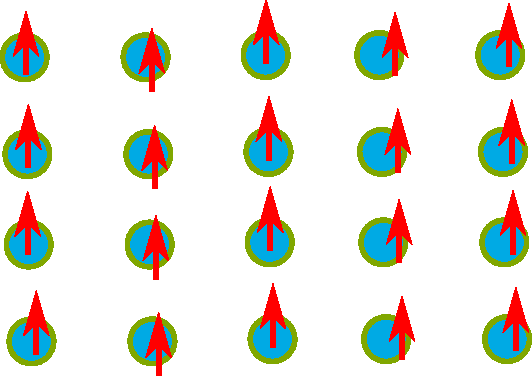
\includegraphics[width=0.7\textwidth]{Tsmall.pdf}
		\caption{$T<T_c$, spins align}
	\end{subfigure}
  \caption{磁子自旋方向随温度变化示意图}\label{fig:ising_two_configurations}
\end{figure}   

\newglossaryentry{ising}{name=伊辛模型, description={Ising model}}
在统计物理学中,\gls{ising}(\glsdesc{ising})指的是
可以处于两种状态的自旋磁子的集合。如图
\ref{fig:ising_two_configurations} 所示,
当外界温度$T$
大于临界温度 $T_c$ 时,
各自旋磁子处于杂乱无章的状态,其总的磁化强度接近0。
但当外界温度$T$
小于临界温度 $T_c$ 时,
各自旋磁子的状态则变得方向一致。
这里,我们称这种方向一致的现象叫自发磁化。

\begin{figure}
	\centering
	\begin{subfigure}{0.45\textwidth}
		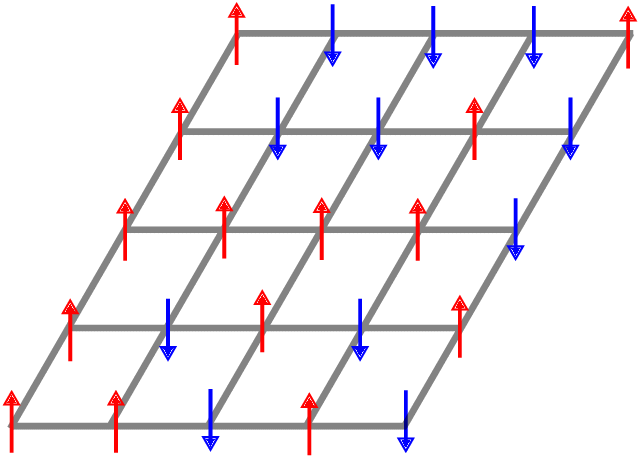
\includegraphics[width=\textwidth]{square-lattice.png}
		\caption{正方形网格}\label{fig:square_lattice}
	\end{subfigure}~
	\begin{subfigure}{0.53\textwidth}
		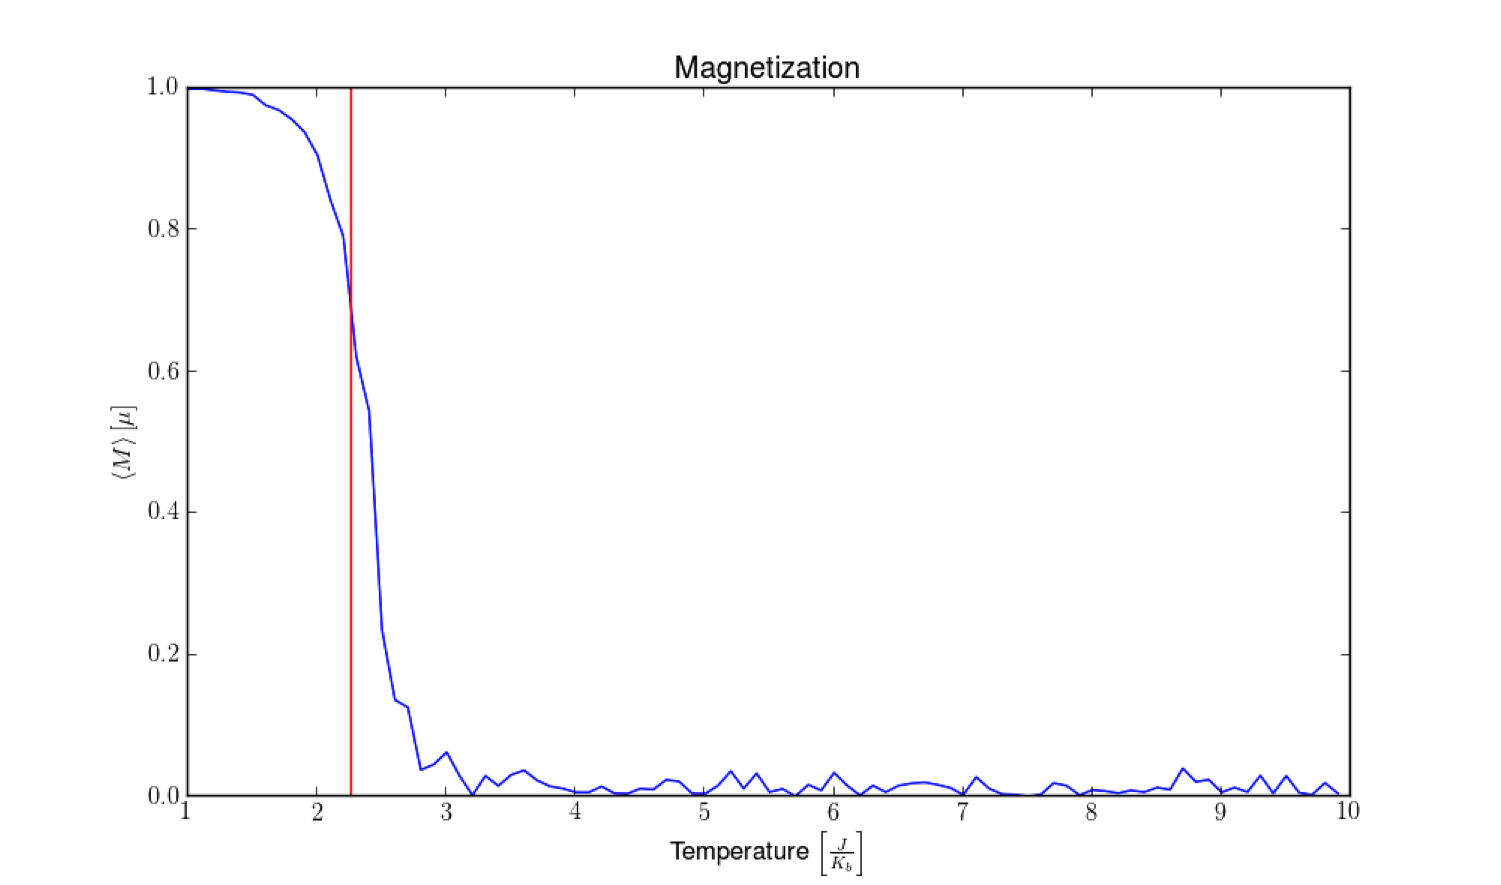
\includegraphics[width=\textwidth]{monte-carlo-ising-6.png}
		\caption{$M$随温度变化情况}\label{fig:square_lattice_b}
	\end{subfigure}
  \caption{正方形网络上的伊辛模型及其磁化强度的变化}
\end{figure}

下面我们介绍伊辛模型一些常用的概念,
如图\ref{fig:square_lattice}所示,
在一个正方形网格中的格点上分布着磁子,一共有$N$个。
$\sigma_i \in \{ \pm 1\} $ 表示第$i$个磁子的状态,
总的磁化强度为 $M = \frac{1}{N} \sum_{i=1}^N \sigma_i$。
理论研究时先考虑有限的正方形网格, 再取 $N\to \infty$。
由于磁子之间的磁力作用和受外场的影响,存在着磁化强度的相变现象,即
\begin{enumerate}
		\item $T< T_c$, $M>0$, 发生自发磁化。
		\item $T> T_c$, $M=0$, 无自发磁化。
\end{enumerate}
图\ref{fig:square_lattice_b}中给出了自发磁化的仿真实验结果,其中临界温度用
红竖线标出。从图中可见在临界温度处磁化强度突然降为零,也即
磁子的自旋方向由完全一致变成两种状态各占一半。我们称临界温度处伊辛模型
\newglossaryentry{phase_trans}{name=相变, description={Phase transition}}
的这种变化为相变(\glsdesc{phase_trans})现象,我们在第\ref{chap:sibm}章也将展示社群发现中也有类似图\ref{fig:square_lattice_b}的相变现象。

对于自发磁化现象可以通过统计力学中的正则系踪(Canonical ensemble)
理论进行解释。该理论
假设粒子的分布为
\begin{equation}\label{eq:canonical_ensemble}
P(\sigma = \bar{\sigma}) = \frac{1}{Z} \exp(-\beta H(\bar{\sigma}))
\end{equation}
其中$\sigma \in \{\pm 1\}^n$ 表示粒子的状态,
$H$叫做汉密尔顿能量函数,表示系统处于状态$\bar{\sigma}$时的总能量,$\beta$是与温度成反比的参数,
\newglossaryentry{inverse_temp}{name=逆温度, description={Thermodynamic beta}}
也叫逆温度(\glsdesc{inverse_temp}),$Z$是配分函数,是概率分布的
归一化常数。

伊辛模型除了定义在正方形网格上外,还可以推广到一般的图 $G(V, E)$ 上。
对于没有外场的情形,伊辛模型的能量函数为
\begin{equation}\label{eq:hamiltonian}
	H(\sigma) = -\sum_{\{i,j\} \in E(G)} \sigma_i \cdot \sigma_j
\end{equation}
在微观层面上,每种微观状态出现的概率均正比于 $\exp(-\beta H(\bar{\sigma}))$,
概率越大或能量越低的状态越有可能出现;在宏观层面则表现为
磁化强度$M$的变化。

\begin{example}
  表 \ref{tab:particles_3} 给出了一个含有3个粒子的系统,其共有8种微观态,
  但根据式\eqref{eq:hamiltonian}, 其在宏观能量的表现了只有$H=-3$或 $H=1$两种组合。
\begin{table}
  \centering
\begin{tabular}{ccc}
		No & Micro state & Macro state ($H$) \\
		1 & $\uparrow\uparrow\uparrow$ & -3 \\
		2 & $\uparrow\uparrow\downarrow$ & 1 \\
		3 & $\uparrow\downarrow\uparrow$ & 1 \\
		4 & $\downarrow\uparrow\uparrow$ & 1 \\
		5 & $\uparrow\downarrow\downarrow$ & 1    \\
6 & $\downarrow\uparrow\downarrow$ & 1 \\
7 & $\downarrow\downarrow\uparrow$ & 1 \\
8 & $\downarrow\downarrow\downarrow$ & -3 \\
\end{tabular}
\caption{一个含有3个粒子的系统的微观状态与宏观能量}
\label{tab:particles_3}
\end{table}
\end{example}

有学者\cite{ye2020exact}
指出,\eqref{eq:hamiltonian} 式所描述的
伊辛模型不存在相变现象,因为式\eqref{eq:canonical_ensemble}
给出的分布聚集在 $\sigma=\pm \mathbf{1}_n$ 附近,
这里 \gls{not:all_one_vector} 表示 \glsdesc{not:all_one_vector}。
\newglossaryentry{not:all_one_vector}
{
  type=notation,
  name={\ensuremath{\mathbf{1}_n}},
  description={长度为 $n$ 的全1的向量}
}
为此,可以采用下述修正模型,将没有边相连的粒子之间的
作用力考虑进来。
\begin{equation}\label{eq:ising_modified}
  H(\bar{\sigma}) = \gamma \frac{\log n}{n} \sum_{\{i,j\}\not\in E(G)}
  \bar{\sigma}_i  \bar{\sigma}_j
	- \sum_{\{i,j\}\in E(G)}
  \bar{\sigma}_i  \bar{\sigma}_j
\end{equation}
这里引入了一个新的参数 $\gamma > 0$。因为该工作研究的是
由随机块模型 $\SSBM(n,2,p,q)$产生的图上定义的伊辛模型,
式\eqref{eq:ising_modified} 出现的系数
$\frac{\log n}{n}$
主要是为了与其研究场景 $p,q=O(\frac{\log n}{n})$
相对应。
\newglossaryentry{metropolis}{name=梅特罗波利斯算法, description={Metropolis algorithm}}

梅特罗波利斯(Metropolis)算法\cite{metropolis1953equation}
用于产生伊辛模型的样本。此外,该算法的变体“模拟退火”
\cite{pincus1970monte} 也是优化领域常用的随机算法。
其算法从系统一个随机的状态出发每次改变其中一个粒子
的状态并按一定的概率接受改变或保持原来的状态。
给定形如式\eqref{eq:ising_modified}
的能量函数,算法\ref{alg:Metropolis}
给出了\gls{metropolis} 的步骤。

\begin{algorithm}
  \caption{梅特罗波利斯算法}\label{alg:Metropolis}
  \begin{algorithmic}[1]
    \STATE 随机初始化 $\bar{\sigma}$
    \STATE 随机选一个粒子进行状态翻转,新的系统状态记为 $\bar{\sigma}'$ 
    \STATE 计算能量差 $\Delta H= H(\bar{\sigma}') - H(\bar{\sigma})$
    \IF{$\Delta H < 0$}
    \STATE $\bar{\sigma} \leftarrow \bar{\sigma}'$
    \ELSE
    \STATE 以概率 $\exp(-\beta \Delta H)$ 
    使得 $\bar{\sigma} \leftarrow \bar{\sigma}'$,
    否则保持原状。 
    \ENDIF
    \STATE 重复步骤 2-8 直到收敛。
\end{algorithmic}  
\end{algorithm}

以上讨论的伊辛模型中粒子均只有$\{\pm 1\}$两个状态,
每个粒子的状态数可以扩展到多个,即 玻茨模型\cite{potts1952some}。
类似式\eqref{eq:hamiltonian},标准玻茨模型的汉密尔顿能量公式为:
\begin{equation}\label{eq:Hsigma_multiple_state}
  H(\sigma) = -\sum_{(i,j) \in E(G)}\delta(\sigma_i, \sigma_j)
\end{equation}
\begin{remark}\label{rem:equivalence_H_energy}
需要注意的是,在状态数$k=2$的情形
式\eqref{eq:Hsigma_multiple_state} 
与式\eqref{eq:hamiltonian}
并不严格等价。
从$\delta(\sigma_i, \sigma_j) = \frac{\sigma_i \sigma_j + 1}{2}$
可以看出,它们之间差了一个伸缩变换。
\end{remark}

\newglossaryentry{sibm}{name=随机块-伊辛模型, description={Stochastic Ising Block Model}}
\newacronym{acr:sibm}{SIBM}{Stochastic Ising Block Model}
将\ref{sec:exact_recovery}小节 介绍的随机块模型与 本小节介绍的 伊辛模型
复合起来可得到 \gls{sibm}(\gls{acr:sibm})\cite{ye2020exact}。
该模型首先由 SBM 生成随机图,
再由随机图上定义的 伊辛模型多次生成节点的状态。
SIBM 模型的恢复任务是由多次生成的节点状态估计节点的真实状态。
该复合模型可用于模拟两党制国家政治选举前的多次民意调查,
生成随机图依据的节点真实状态即为选民
的政治倾向。下面对SIBM的研究结果进行简要介绍。

在\citet{ye2020exact} 的研究工作中,由 $\SSBM(n,2,\A, \B)$
生成随机图,采用 \eqref{eq:ising_modified} 定义的能量函数
独立生成 伊辛模型的样本 $m$ 次,记为
$\SIBM(n, \A, \B, \gamma, \beta, m)$。
类似 \ref{sec:exact_recovery}节
针对SBM的精确恢复,
同样在 SIBM 上也可以定义精确恢复为:
\begin{definition}\label{def:sibm_exact_recovery}
  设 $(\sigma^{(1)}, \dots, \sigma^{(m)})$
  由 $\SIBM(n, \A, \B, \gamma, \beta, m)$ 生成。
  称该 SIBM 可精确恢复,如果存在算法$\hat{X}$以
  $(\sigma^{(1)}, \dots, \sigma^{(m)})$ 为输入,
  满足 $\lim_{n\to \infty}P(\hat{X}=\pm X) = 1$。 
\end{definition}

类似 SBM,SIBM 也存在相变现象,可总结为如下的定理。
\begin{theorem}\label{thm:sibm_phase_trans}
  设 $\sqrt{a} - \sqrt{b} > \sqrt{2}$ 且 $\gamma, \beta > 0$,
  定义临界量 $\beta^*, m^*$ 为:
  \begin{equation}\label{eq:beta_star_sibm}
    \beta^* :=  \frac{1}{2} \log \frac{a+b-2 - \sqrt{(a+b-2)^2-4ab}}{2b}
    \, \textrm{ 和 } \,
    m^* := 2\left\lfloor\frac{\beta^*}{\beta} \right\rfloor + 1
  \end{equation}
  针对 $\SIBM(n, \A, \B, \gamma, \beta, m)$ 模型,我们有
  \newglossaryentry{not:small_o}
{
  type=notation,
  name={$o(1)$},
  description={无穷小量}
}
  \begin{enumerate}
    \item\label{enu:m_larger} 若 $\gamma > b, m \geq m^*$,SIBM 可精确恢复;
    \item\label{enu:m_smaller} 若 $\gamma >b, m < m^*-2$,当$n\to \infty$ 时,所有SIBM 恢复算法的成功率趋近于零;
    \item\label{enu:gamma_b} 若 $ \gamma < b$, 则 $ m = O(\log^{1/4}(n))$,故 SIBM无法精确恢复,特别地,对于$m$是不随$n$
    增长的常数时 SIBM 无法精确恢复;
    \item\label{enu:beta_larger}  若 $\gamma>b, m=1, \beta > \beta^*$,则 $P(\sigma^{(1)}=\pm X) = 1-$\gls{not:small_o};
    \item\label{enu:beta_smaller}  若 $\gamma>b, m=1, \beta \leq \beta^*$,则
    $P(\Dist(\sigma^{(1)}, \pm X) =
    \Theta(n^{g(\beta)}))=1-o(1)$。
  \end{enumerate}
  这里, $g(\beta)$ 函数定义为
  \begin{equation}
    g(\beta):= \frac{be^{2\beta} + a e^{-2\beta}}{2} - \frac{a+b}{2} +1
  \end{equation}
\end{theorem}
在定理 \ref{thm:sibm_phase_trans} 中,
注意到 $\sqrt{a} - \sqrt{b} > \sqrt{2}$ 的条件保证了
式\ref{eq:beta_star_sibm} 中根号下的项非负。
另外定理\ref{thm:sibm_phase_trans} 中\ref{enu:beta_larger}、\ref{enu:beta_smaller}
两点讨论的是从随机图中产生一个样本的情况,
说明了$\beta^*$ 是一个临界值点。当$\beta>\beta^*$ 时,
使用 伊辛模型(可看作社群发现的随机算法)产生的样本恢复随机块模型各节点的真实标签
可实现精确恢复(参见定义\ref{def:SSBMR})。
而当$\beta\leq \beta^*$ 时, 伊辛样本与真实标签的距离是随$n$增长的,
说明精确恢复不可实现。

\citet{ye2020exact} 的工作中关注的重点是对采样数量$m$的相变现象的讨论,
在采多个样本的情况下,定理\ref{thm:sibm_phase_trans} 中\ref{enu:m_larger}、\ref{enu:m_smaller}
两点说明存在一个相对于定义\ref{def:sibm_exact_recovery}给出的精确恢复的临界值$m^*$。
最后,定理\ref{thm:sibm_phase_trans} 中
的第\ref{enu:gamma_b}点
说明$\gamma>b$
是精确恢复的前提。
如果$\gamma<b$,则
伊辛模型产生的样本
相比于$\pm X$的位置
会以更大的概率聚集在$\pm \bm{1}$。


\citet{ye2020exact} 在本工作的技术证明中,用到了马尔可夫不等式和切尔诺夫不等式这两个概率论中常用的聚集不等式。
由于我们在后面章节的技术证明中也要用到这两个不等式,故在本小节最后列出它们,方便后面引用。

\newglossaryentry{markov_ieq}{name=马尔可夫不等式, description={Markov Inequality}}
\begin{lemma}[\gls{markov_ieq}] 
  设 $X$ 是非负型随机变量,则对于非负实数$a$有:
  \begin{equation}
    P(X\geq a) \leq {1 \over a} \E[X]   
  \end{equation}
   若$X$ 不一定非负,$a$ 是任意实数,可先取$e$指数再运用马尔可夫不等式,
   即有
   \begin{equation}\label{eq:chernoff_bound}
    P(X\geq a) = P(e^{tX} \geq e^{ta}) \leq { 1 \over \exp(ta)} \E[\exp(tX)]
   \end{equation}
   对任意的$t>0$成立。
   \newglossaryentry{chernoff}{name=切尔诺夫不等式, description={Chernoff Inequality}}

   式\eqref{eq:chernoff_bound}也被称为 \gls{chernoff}。
\end{lemma}
\newglossaryentry{chebyshev_ieq}{name=切比雪夫不等式, 
description={Chebyshev's Inequality}}
\begin{lemma}[\gls{chebyshev_ieq}]
  \newglossaryentry{not:variance}
{
  type=notation,
  name={$\Var[\cdot]$},
  description={方差}
}
  对于随机变量 $X$, 正实数$a$,我们有
  \begin{equation}
    P(\abs{X-\E[X]} \geq a) \leq {1 \over a^2} \Var[X]
  \end{equation}
  这里,$\Var[X]$表示随机变量$X$的\glsdesc{not:variance}。
\end{lemma}

% to do: add large deviation theory and hypothesis testing


\subsection{最大模块度算法与基于半正定规划的社群发现算法}

最后,我们再简单介绍一下社群发现领域常用的最大模块度算法
\cite{newman2006modularity}。
\newglossaryentry{modularity}{name=模块度, description={Modularity}}
\gls{modularity}(\glsdesc{modularity})
是对网络结构或图结构的一种度量,既能作为评价指标评价
不同社群发现算法的性能,也能通过近似求解模块度最大值的思路设计算法。
模板度越高,则节点集内部连接越紧密,而节点集之间连接越稀疏。

给定$n$长的向量$x$,模块度的数学定义为:
\begin{align}\label{eq:Q}
  Q(x) &= \frac{1}{2 |E|} \sum_{ij} (A_{ij} - \frac{d_i d_j}{2 |E|}) \delta(x_i, x_j)
\end{align}
这里 $A$ 表示图的邻接矩阵,$|E|$表示边的数量,
而$d_i$表示第
\newglossaryentry{degree}{name=度, description={Degree}}
$i$个节点的\gls{degree}(\glsdesc{degree}),$x_i$ 表示第$i$
个节点所属的社群。

贪心法是用于近似求解式\eqref{eq:Q}
近似求解最大值的常用算法,其流程类似于系统聚类法,
即从每个节点各自属于一类出发,通过中间指标最大的方法每次聚合两类,
使得 $Q$ 不断增大。该思路可经过优化适用于求解大规模网络
的社群发现问题 \cite{clauset2004finding}。


针对随机块模型的社群发现
可以先将最大似然方法获得的目标函数
写成整数优化的问题形式,
\newacronym{acr:sdp}{SDP}{Semi-definite programming}
\newglossaryentry{sdp}{name=半正定规划, description={Semi-definite programming}}
再转化成半正定规划 (\gls{acr:sdp}) 的优化问题进行求解。

在 式\eqref{eq:minimum_k_cut} 中
取 $\delta(y_i, y_j) = \frac{1+y_iy_j}{2}$,
于是可得到如下
的优化问题:
\begin{align}
  \max_x\, &  x^T A x \notag \\
  \textrm{s.t. } & x_{i} = 1, i \in [n] \notag \\
  & \mathbf{1}^T x = 0
\end{align}
其中 $A$ 表示图的邻接矩阵。
$ x^T A x $ 可以看成是 $\langle xx^T, A \rangle $,即矩阵
\newglossaryentry{not:matrix_inner_product}
{
  type=notation,
  name={$\langle A, B \rangle $},
  description={矩阵$A$ 和 $B$ 的内积}
}
$xx^T$ 与 $A$ 的内积。令$Y=xx^T$,则$Y$是一个
半正定的矩阵,若对$Y$秩为1的条件进行松弛,则
得到如下半正定规划问题:
\begin{align}\label{eq:opt_A_Y_1}
  \max_Y\, & \langle A, Y \rangle  \notag \\
  \textrm{s.t. } & Y_{ii} = 1, i \in [n] \notag \\
  & \langle Y, J_n \rangle  = 0
\end{align}
\newglossaryentry{not:matrix_all_one}
{
  type=notation,
  name={$J_n$},
  description={元素全为1的$n\times n$的矩阵}
}
其中 $J_n=\mathbf{1}_n\mathbf{1}_n^T$
是 \glsdesc{not:matrix_all_one}。
令 $B=2A + I_n - J_n$,
\newglossaryentry{not:identity_matrix}
{
  type=notation,
  name={$I_n$},
  description={$n\times n$的单位矩阵}
}
$I_n$ 是 \glsdesc{not:identity_matrix},
则
优化的目标函数还可写成 $ \langle B, Y \rangle $,
其中 $B$的定义为
\begin{equation}\label{eq:def_B_sdp}
    B_{ij} = \begin{cases}
        1, & \text{若 $i$ 与 $j$ 相连}, \\
        -1,& \text{否则}
    \end{cases}
\end{equation}  

以上方法可针对一般的图$G$进行求解,
但对于$\SSBM(n,2, \A, \B)$,
Hajek 等学者 \cite{hajek2016achieving} 得到了SDP做社群发现的
理论保证。
\begin{theorem}
  设 $\hat{Y}$ 是
  优化问题 \eqref{eq:opt_A_Y_1} 的解, $\sigma$ 是节点的真实标签向量。
  若 $\sqrt{a} - \sqrt{b}
  > \sqrt{2}$,
  则
  $\lim_{n\to\infty} P(\hat{Y}=\sigma\sigma^T)=1$。
\end{theorem}
\section{信息论度量}
由于本文要用到多种信息论度量研究
社群发现问题,下面依次对多变量互信息、速率函数、雷尼散度等相关知识进行简要介绍。

\subsection{多变量互信息与局部信息几何}\label{sec:local_geometry}
\subsection{信息聚类}\label{sec:info_clustering}
在信息论领域,互信息提供了两个随机变量之间的
距离度量。使用 KL 散度的记号,随机变量$X$
和 $Y$ 之间的互信息定义为:
\begin{equation}\label{eq:mutual_info}
  I(X;Y) = D(P_{XY} ||P_XP_Y)
\end{equation}
\newglossaryentry{not:kl_dev}
{
  type=notation,
  name={$D(P_X||P_Y)$},
  description={分布$P_X$ 和 $P_Y$之间的 KL 散度}
}
其中 $P_X, P_Y$分别表示边缘分布,$D(P_X||P_Y)$
表示 \glsdesc{not:kl_dev}。
而$P_{XY}$
表示两个随机变量的联合分布。有多种方法可将互信息
的概念推广到两个及以上的随机变量,
其中华人学者陈聪提出了一种推广 \cite{ska} 具有多种好的性质,
\newglossaryentry{mmi}{name=多变量互信息, description={Multivariate mutual information}}
\newacronym{acr:mmi}{MMI}{Multivariate mutual information}
且涵盖了图结构的情形,我们把他的推广叫做 \gls{mmi} (\gls{acr:mmi})。

下面我们对MMI做简要的介绍。定义$V$是随机变量
的序号集合,$C$是 $V$的子集,$Z_C=\{Z_i | i \in C\}$
表示随机变量序号在 $C$ 中的随机变量 $Z_i$ 的集合。
$\P$ 表示$V$ 的一个分割,$P_{Z_C}$表示$Z_C$
的联合分布。$\Pi'(V)$ 是
除去$\{V\}$外所有$V$的分割的集合。MMI的度量定义为:
\begin{align}
  I(Z_V) &:= \min_{\P \in \Pi'(V)} I_{\P}(Z_V)
  \textrm{ 其中 } \label{eq:IZV}\\  
  I_{\P}(Z_V) &:= \frac{1}{|\P| - 1}D(P_{Z_V} || \prod_{C\in \P} P_{Z_C}) \label{eq:IPZV}
\end{align}
在上面的定义中,如果$Z_V$彼此独立,那么$I(Z_V)=0$,
反之亦然。

式\eqref{eq:IPZV}给出了特定分割下的多变量互信息,
也可根据下式把KL散度改写成熵的形式。
\begin{equation}\label{eq:entropy_expression}
  D(P_{Z_V} || \prod_{C\in \P} P_{Z_C}) 
  = \sum_{C \in \P}
  H(Z_C) - H(Z_V)
\end{equation}
对于一般的分布,式\ref{eq:IZV}
难于计算。陈聪提出了一种特殊的PIN模型\cite{pin}\footnote{PIN 是 pairewise independent network
的缩写},
使得多变量互信息可以用\ref{sec:community_detection}节
介绍的PSP算法进行计算。
这里略去PIN模型的数学定义,而是通过下面的例子
阐发它和图结构的联系。
\begin{example}\label{ex:mmi}
  令$V=\{1,2,3\}$,$Z_1=(X_a, X_c)$,
  $Z_2=(X_a,X_b)$ 且 $Z_3=(X_b,X_c)$。
  $X_a,X_b,X_c$是独立的随机变量且它们的熵分别为:
  $H(X_a)=H(X_b)=1, H(X_c)=5$。
  利用联合熵的公式不难计算出$H(Z_1)=H(X_a)+H(X_c)$以及
  $H(Z_1, Z_2) = H(X_a) + H(X_b) + H(X_c)$等。
  若 $\P=\{\{1,2\}, \{3\}\}$,则根据
  \eqref{eq:entropy_expression}式,
  $D(P_{Z_V}||P_{Z_1,Z_2}P_{Z_3}) = H(X_a)
  +H(X_b)$。我们可以将上面的计算用图\ref{fig:example_directed}
  进行对应,即把$Z_i$对应到第$i$的节点,
  $Z_i$与$Z_j$之间的互信息对应到第$i$和第$j$个节点之间
  边的权值,而KL散度即为不同的类别之间边的权值之和。
\end{example}
例\ref{ex:mmi}中虽然只有三个节点,
但对于一般的情形,PIN模型也是和一个有向图有
着类似的对应关系。因此,在PIN模型下多变量互信息可以用
PSP算法进行计算。

基于MMI可以对随机变量进行聚类,聚类簇
定义为
\begin{align}
  C(Z_V) &:= \bigcup_{\gamma \in \R} C_{\gamma}(Z_V)
  \label{eq:czv}\\
  C_{\gamma}(Z_V) &:= \textrm{maximal}
  \{ B \subseteq V \big\vert |B|>1, I(Z_B) > \gamma  \}
\end{align}
理论分析表明,基于定义式\ref{eq:czv} 可以得到和
式\ref{eq:PSP_structure}类似的层次聚类结果。
即存在一系列的临界值$\lambda_1 < \dots < \lambda_k$和分割
$\P_k \preceq \dots \preceq \P_0$,使得
$C(Z_V) = \bigcup_{i=1}^{k} C_{\lambda_i}(Z_V)$
且$C_{\lambda_i}(Z_V) = \P_i$。

有两种生成聚类簇的方法 \cite{chan2020agglomerative},它们均可以通过聚类树
来描述。聚类树可看成是一系列
嵌套的分割$\P_i$的另一种描述方式。
聚类树有一个根节点$V$,
其所有的叶节点为 $\{j\}$,其他节点均对应着
一个聚类簇。

\begin{description}
  \item[自顶向下] 假设 $I_{\P^*}(Z_V)=I(Z_V)$, 
  把 $\P^*$ 中每一个元素作为 $V$ 的子节点。
  对于每一个子节点$C$,求解$I(Z_C)=I_{\P_C}(Z_C)$
  并使用分割 $\P_C$ 对子树进一步细分直到子节点变成单元素集为止。
  \item[自底向上\footnotemark] 假设 $I(Z_C) = \max_{B\subseteq V} I(Z_B)$ 并且 
  将 $C$ 中所有的元素合并成一个作为聚类树的子节点。对于当前所有子节点,找到MMI
  最大的集合进行合并直到所有子节点合并成根节点$V$为止。
  \end{description}
  \footnotetext{参见\cite{agg_ic}}

  \begin{figure}[!ht]
    \centering
    \begin{subfigure}[b]{0.38\linewidth}
      \centering
      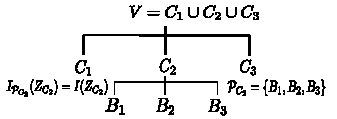
\includegraphics[width=\textwidth]{top_down.pdf}
      \caption{}\label{fig:top_down}
    \end{subfigure}~
  \begin{subfigure}[b]{0.33\linewidth}
    \centering
    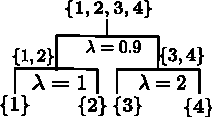
\includegraphics[width=\textwidth]{threshold_a.pdf}
    \caption{}\label{fig:threshold_a}
  \end{subfigure}~
  \begin{subfigure}[b]{0.29\linewidth}
    \centering
    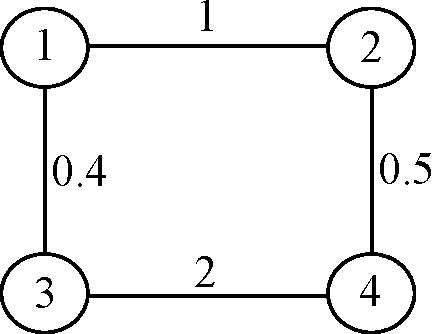
\includegraphics[width=\textwidth]{threshold_b.pdf}
    \caption{}\label{fig:threshold_b}
  \end{subfigure}
    \caption{聚类树示例}\label{fig:mmi_example}
  \end{figure}
自顶向下
获得聚类树的示意图由图 \ref{fig:top_down} 给出。
下面我们用一个简单的例子来说明聚类树的结构。
  \begin{example}\label{ex:mmi_tree}
考虑图\ref{fig:threshold_b}所示的情形,
$V=\{1,2,3,4\}$。互信息在图的边上标出,
比如 $I(Z_1;Z_2)=1, I(Z_1;Z_4)=0$。
利用定义式\ref{eq:IZV}不难求出
$I(Z_V)=0.9$。 
我们可以写出完整的聚类结果:
\begin{equation*}
\P = 
\begin{cases}
\{\{1,2,3,4\}\} & \lambda < 0.9 \\
\{\{1,2\},\{3,4\}\} & 0.9 \leq \lambda < 1 \\
\{\{1\},\{2\},\{3,4\}\} & 1 \leq \lambda < 2\\
\{\{1\},\{2\},\{3\},\{4\}\} & \lambda \geq 2
\end{cases}
\end{equation*}
把各临界值$\lambda_i$ 标到聚类树上即如图
\ref{fig:threshold_a}所示。
\end{example}
最后,我们再介绍一个多变量互信息的性质,它将在我们后面社群中的异常值点的检测工作中
用到。这个性质给出了最大的临界值 $\lambda_k$ 的多变量互信息表达式\cite{agg_ic}:
\begin{equation}\label{eq:largest_threshold}
\lambda_k = \max_{A\subseteq V} I(Z_A)
\end{equation}

局部信息几何的理论是由华人学者郑立中等人提出\cite{huang2019universal},
可从理论的层面分析机器学习中的特征提取\cite{huang2017information}、人工神经网络
\cite{huang2019information}等问题。
下面对本工作中用到的局部信息几何的内容进行简要的介绍。

KL散度可用于度量两种不同概率分布
之间的距离。当这两种分布比较接近时,
局部信息几何刻画了KL散度的近似表达式。
我们以离散分布为例,给出分布之间距离的接近的
形式化定义。
$P_0$ 表示一概率质量函数 (Probability mass function),
其定义域为字母集$\mathcal{X}$,
$\epsilon$表示一无穷小量。
\begin{definition}\label{def:eps_neighborhood}
我们称 $P$ 在 $P_0$的 $\epsilon$ 邻域 $N^{(\epsilon)}(P_0)$ 内,如果
\begin{equation}\label{eq:P_neighborhood}
P \in N^{(\epsilon)}(P_0) \iff
\sum_{x \in \mathcal{X}} \frac{(P(x) - P_0(x))^2}{P_0(x)} \leq \epsilon^2
\end{equation}
\end{definition}
式\eqref{eq:P_neighborhood}可以写成 $P(x) = P_0(x) + \epsilon
\sqrt{P_0(x)} \phi(x) + o(\epsilon)$的简化形式, 其中 $\phi(x)$
叫做特征函数,它的欧氏范数 $||\phi || $ 不超过1。
对于两个在$P_0$的$\epsilon$邻域内的分布 $P_1, P_2$,我们有
\begin{equation}\label{eq:approx:ig}
D(P_1 || P_2) = \frac{\epsilon^2}{2} ||\phi_1 - \phi_2||^2 + o(\epsilon^2)
\end{equation}
对于两个弱独立的随机变量,也有类似式\ref{eq:approx:ig}
的结论。
\begin{definition}\label{def:weak_indepedent}
我们称 $X$ 和 $Y$ 是 $\epsilon$-\textbf{弱独立}的,
如果 对于任何 $x \in \mathcal{X}$,
$Y$关于$X$的条件分布
$P_{Y|X}(\cdot |x)$在$Y$的$\epsilon$邻域内。
\end{definition}
在弱独立的假设下, 由 $D(P_{XY}||P_XP_Y)$ 所定义的互信息$I(X;Y)$, 
通过对式\eqref{eq:approx:ig}的化简,可以表示为:
\begin{equation}\label{eq:Ixy}
I(X;Y) = \frac{1}{2}\sum_{x\in \mathcal{X}, y\in \mathcal{Y}} B^2(x,y) + o(\epsilon^2)
\textrm{ 其中 }  B(x,y)=\frac{P_{X,Y}(x,y) - P_X(x) P_Y(y)}{\sqrt{P_X(x)P_Y(y)}}
\end{equation}
在式\eqref{eq:Ixy}中, $\sum_{x\in \mathcal{X}, y\in \mathcal{Y}} B^2(x,y)$
一项可以写成 $\norm{B}_F^2$。这里 $B$表示$\mathcal{X} \times \mathcal{Y}$的矩阵,
\newglossaryentry{not:norm_f}
{
  type=notation,
  name={$||\cdot||_F$},
  description={矩阵的Frobenius范数}
}
$F$表示 \glsdesc{not:norm_f}。
Equation \eqref{eq:Ixy} 表明,当$X$和$Y$弱独立时,
$I(X;Y)$可用$\frac{1}{2} \norm{B}_F^2$
近似,其阶数为 $O(\epsilon^2)$。

\begin{example}\label{ex:Pweak_1}
考虑 $P_0=(X_0,Y_0)$是一个两维的随机向量,
$P_0(x,y)=\frac{1}{4}$ 对于$x,y \in \{0,1\}$。
不然发现$X_0,Y_0$
是独立同分布的伯努利随机变量。
定义 $P(x,y)=\frac{1}{4}(1+\epsilon (-1)^{x+y})$,
则 $P\in N^{(\epsilon)}(P_0)$,而
$\phi(x,y) = \frac{(-1)^{x+y}}{2}$
且有 $||\phi||=1$。
利用 $\log(1+x) = x - \frac{1}{2}x^2 + o(x^2)$
不难得到 $D(P_0||P)=\frac{\epsilon^2}{2}
+o(\epsilon^2)$,从而印证了
式\eqref{eq:approx:ig}的结论。
此外,根据定义\ref{def:weak_indepedent}
我们可以验证$X$与$Y$是弱独立的。
这里,$X,Y$表示分布$\frac{1}{4}(1+\epsilon (-1)^{x+y})$
的两个维度。由式\eqref{eq:Ixy}计算出
$I(X;Y)=\frac{1}{2}\epsilon^2+o(\epsilon^2)$
与从互信息的定义式出发计算得到的结果相同,
从而印证
了弱独立情形下互信息的表达式。
\end{example}

\subsection{速率函数与大偏差原理}
本小节将首先从型的概念出发,引出针对离散随机变量的大偏差原理:Sanov定理,
型的概念和Sanov定理将在我们推导拓展随机块模型的最优误差率结论中用到。之后我们会
介绍大偏差原理的一般形式,即Cramér定理,从而引出速率函数的概念。

\newglossaryentry{type}{name=型, description={Type}}
在信息论中,我们首先假定所有的元素均从字母集$\mathcal{X}$
中选取。
某个长度为$n$序列$x$的 \gls{type} 是表示
各字符在该序列中出现的比例,用符号$P_x$表示,
所有的$P_x$组成集合$\P_n$。比如考虑字母集
$\mathcal{X}=\{1,2,3\}$。对于$11321$
它的型可以用三元组 $(\frac{3}{5}, 
\frac{1}{5}, \frac{1}{5})$ 表示。注意到
一个型对应着一个离散分布的概率质量函数。

假设 长度为$n$序列$x=(x_1,\dots, x_n)$中每个元素 都是 i.i.d. 服从分布 $Q(x)$,
则它的联合分布的概率质量函数可以记为$Q^n(x)=\prod_{i=1}^n x_i$。
对于任意长度为$n$的序列$x$,我们仍沿用上述关于$Q(x)$的定义。
为衡量$Q$和另一个不包括$Q$的概率分布的集合 $E$ 之间的距离,我们引入如下的记号:
$Q^n(E) = \sum_{x: P_x \in E \cap \P_n} Q^n(x)$。
这里 $P_x$ 是 $x$的型。

下面介绍的 Sanov 定理给出了$Q^n(E)$的上下界:
\begin{theorem}
  设 $X_1, \dots, X_n$ i.i.d. 服从分布 $Q(x)$,
  若 $E$ 表示概率分布的集合,且$E$的闭包是其自身。
  则
  \begin{equation}
  \frac{1}{(n+1)^{|\mathcal{X}|}} e^{-n D(P^*||Q)}
  \leq Q^n(E) \leq (n+1)^{|\mathcal{X}|} e^{-n D(P^*||Q)}
  \end{equation}
  其中
  \begin{equation}
    P^* = \arg\min_{P\in E} D(P||Q)
  \end{equation}
  极限情形下有:
  \begin{equation}\label{eq:limit_sanov}
    \lim_{n\to \infty} \frac{1}{n} \log Q^n(E) = -D(P^*||Q)
  \end{equation}
\end{theorem}
\begin{example}\label{ex:sanov_ldp}
若$X_1, \dots, X_n$ i.i.d. $\sim \Bern(p)$,
对于任意正数$\epsilon$,
我们可以用 Sanov 定理估计 $P(\frac{1}{n} \sum_{i=1}^n X_i > \bar{X} + \epsilon)$ 随着$n$增大收敛到零
的速率,其中$\bar{X}$是$X_1,\dots, X_n$的平均值,等于$p$。
此时集合$E=\{\Bern(q)| q>p+\epsilon\}$。
而$Q^n(E)=P(\frac{1}{n} \sum_{i=1}^n X_i > \bar{X} + \epsilon)$
因此由式\eqref{eq:limit_sanov}可得 $\lim_{n\to \infty} \frac{1}{n} \log Q^n(E)=-D(\Bern(p+\epsilon)||\Bern(p))$。
\end{example}
Sanov 定理仅针对离散型分布给出了计算诸如
的方法,若将例\ref{ex:sanov_ldp} 中诸$X_i$ 改为高斯分布,
则可以用Sanov 定理的推广形式 Cramér定理来解决。我们下面先介绍该定理:

\begin{theorem}\label{thm:cramer}
  \newglossaryentry{log_mgf}{name=对数矩生成函数, description={logarithmic moment generating function}}
  \newacronym{acr:log_mgf}{log-MGF}{logarithmic moment generating function}
  令 $X_i$ 为i.i.d. 的随机变量序列,且$X_1$ 存在 \gls{log_mgf} (\gls{acr:log_mgf})
$\Lambda(t)=\log \E[\exp(t X_1)]$。
令 $\Lambda^*(s)= \sup_{t \in \R} st-\Lambda(t)$,则对于所有$s>\E[X_1]$,
我们有
\begin{equation}\label{eq:cramer}
\lim_{n\to \infty} \frac{1}{n}\log P( \sum_{i=1}^n X_i \geq  ns) = - \Lambda^*(s)
\end{equation}
\end{theorem}
由于$\Lambda^*(s)$描述了$P( \sum_{i=1}^n X_i \geq  ns)$随$n$增大衰减到零的速率,
\newglossaryentry{rate_function}{name=速率函数, description={rate function}}
我们把$\Lambda^*(s)$叫做 \gls{rate_function}。

为方便描述,$\Lambda^*(s)$和$\Lambda(s)$的关系,
我们引入凸共轭函数的概念。
\begin{definition}
  定义在$\R$ 上的光滑函数 $\Lambda(s)$,
  它的凸共轭函数定义为
  $\Lambda^*(s) = \sup_{t \in \R} st-\Lambda(t)$。
  $\Lambda^*(s)$ 再取一次凸共轭又得到 $\Lambda(s)$自身。    
\end{definition}

\begin{example}\label{ex:cramer_ldp}
  若$X_1, \dots, X_n$ i.i.d. $\sim \mathcal{N}(0,1)$,
  对于任意正数$\epsilon$,
  下面我们 用  Cramér 定理 计算 $P(\frac{1}{n} \sum_{i=1}^n X_i > \epsilon)$ 
  随着$n$增大收敛到零
  的速率。首先计算标准正态分布的 log-MGF 为 $\Lambda(s)=s^2/2$,
  其凸共轭$\Lambda^*(s)=\Lambda(s)=s^2/2$。因此
  由式\eqref{eq:cramer}
  $\lim_{n\to \infty} \frac{1}{n}\log P( \sum_{i=1}^n X_i \geq  ns) =-s^2/2$。
  \end{example}

\subsection{雷尼散度与切尔诺夫信息}
在假设检验的问题中,我们要确定 i.i.d. 采样的样本
$X_1, \dots, X_n$ 服从
$P_1$ 还是 $P_2$ 分布。为此,考虑两个假设:
$H_1: Q=P_1$ 和 $H_2: Q=P_2$。
决策变量$\widehat{H}$ 的值域为 $\{P_1, P_2\}$。
在做决策的时候可能会产生两类错误,它们的概率
分别是 $\alpha_n=P(\widehat{H}=H_2|H_1)$
以及 $\beta_n=P(\widehat{H}=H_1|H_2)$。
这里下标 $n$表明错误概率随采样数量$n$而变化。
假设$P_1, P_2$的先验概率分别是 $\pi_1$ 和 $\pi_2$,
则总误差概率为:$P_e^{(n)} = \pi_1 \alpha_n
+ \pi_2 \beta_n$。

\newglossaryentry{error_exponent}{name=误差指数, description={error exponent}}
$P_e^{(n)}$ 和决策变量$\widehat{H}$的选取有关。
切尔诺夫信息指出了在渐近情形下 $P_e^{(n)}$ 所能达到的
最小值,更精确的说,最大的误差指数。因为
在这种情形下 $P_e^{(n)}$ 以 $\exp(-n D^*)$ 的速率指数衰减。
我们把$D^*$叫做 \gls{error_exponent}。
$D^*$的数学定义为:
\begin{equation}
 D^* = \lim_{n\to \infty} -\frac{1}{n} \min_{\widehat{H}}
 P^{(n)}_e
\end{equation}
关于 $D^*$ 我们有如下定理\footnote{关于此定理可参考\citet{cover1999elements}的教科书
11.9 节}:
\begin{theorem}
  \newglossaryentry{chernoff_information}{name=切尔诺夫信息, description={Chernoff Information}}
  最大误差指数 $D^*$,也称\gls{chernoff_information}, 满足
  \begin{equation}\label{eq:D_star_lambda_star}
    D^* = D(P_{\lambda^*} || P_1) = D(P_{\lambda^*}|| P_2)
  \end{equation}
  而 $P_{\lambda}$ 定义为
  \begin{equation}\label{eq:P_lambda_x}
    P_{\lambda}(x) = \frac{P^{1-\lambda}_1 (x) P^{\lambda}_2 (x)}
    {\sum_{a \in \mathcal{X}} P^{1-\lambda}_1 (a) P^{\lambda}_2 (a)}
  \end{equation}
  $\lambda^*$ 的取值使得  \eqref{eq:D_star_lambda_star} 式成立。
\end{theorem}

\newglossaryentry{not:chernoff_information}
{
  type=notation,
  name={$C(P_1||P_2)$},
  description={分布$P_1$和$P_2$之间的切尔诺夫信息}
}
为方便讨论,我们使用符号$C(P_1||P_2)$
来表示\glsdesc{not:chernoff_information}。

切尔诺夫信息的另一个等价定义是:
\begin{equation}\label{eq:C_P_1_P_2_another}
  C(P_1||P_2) = -\min_{0\leq \lambda \leq 1}
  \log \left(\sum_{x \in \mathcal{X}}
  P^{1-\lambda}_1(x)P^{\lambda}_2(x)
  \right)
\end{equation}

当我们考虑联合分布 $P_1 \times P_2$
和 $P_2 \times P_1$ 之间的切尔诺夫信息量时,
由式 \eqref{eq:C_P_1_P_2_another}
\begin{align*}
  C(P_1 \times P_2||P_2 \times P_1) 
  = -\min_{\lambda \in [0,1]}
  \left(\log \sum_{x\in \mathcal{X}}
  P_1^{1-\lambda}(x) P_2^{\lambda}(x) 
  +\log \sum_{y\in \mathcal{X}}
  P_2^{1-\lambda}(y) P_1^{\lambda}(y) 
  \right)
  \end{align*}
该目标函数在$\lambda=\frac{1}{2}$
处一阶导数为零而二阶导数为正,因此最小值
在$\lambda=\frac{1}{2}$取到。该最小值
即为阶数为$\frac{1}{2}$的 \gls{renyi_divergence}。
\newglossaryentry{renyi_divergence}{name=雷尼散度, description={Rényi divergence}}
记为:
\begin{equation}\label{eq:renyi_divergence}
  D_{1/2}(P_1 || P_2) = C(P_1 \times P_2||P_2 \times P_1)=
  -2\log \left(\sum_{x \in \mathcal{X}}
  \sqrt{P_1(x)P_2(x)} \right)
\end{equation}

雷尼散度在刻画一些SBM模型及其变体的误差衰减
速率时常常用到 \cite{zhang2016}。
比如在两社群的SBM模型中,我们取$P_1=\Pois(\frac{a}{2}),P_2=\Pois(\frac{b}{2})$
代入式 \eqref{eq:renyi_divergence} 
得
\begin{equation}
  D_{1/2}(\Pois(\frac{a}{2}) || \Pois(\frac{b}{2}))
  = \frac{1}{2}(\sqrt{a} - \sqrt{b})^2
\end{equation}

%\subsection{小节}
以上介绍的三种度量都可以看做KL散度的某种推广,在实际使用中根据所研究
的问题选取较为方便的度量形式更易获得有启发性的结论,
这一点我们将在后面的章节进行具体阐示。
